%% Requires compilation with XeLaTeX or LuaLaTeX
\documentclass[10pt,xcolor={table,dvipsnames},t]{beamer}

\usepackage[spanish]{babel}
\usepackage{amssymb}

\title{Auómatas para la vinculación parcial de servicios}
% \subtitle{Your subtitle (if there's one)}
\author{Ezequiel Davidovich Caballero}
\institute{Departamento de Computación, Facultad de Ciencias Exactas y Naturales}
\date{11 de Noviembre 2020}


\begin{document}


\begin{frame}
\vspace{-2cm}
\begin{center}
\begin{tabular}{l}

\includegraphics[width=2cm]{logofcen.pdf}
\end{tabular}    
\end{center}

  \titlepage
  
  {

{Director: Carlos G. Lopez Pombo}

\vspace{.2cm}

{Codirector: Ignacio Vissani}

\vspace{.2cm}

Buenos Aires, 2020
}
\end{frame}

% Uncomment these lines for an automatically generated outline.
%\begin{frame}{Outline}
%  \tableofcontents
%\end{frame}

\section{Introduction}

\begin{frame}{Service-oriented Computing}

Service-oriented computing (SOC) es el paradigma de cómputo que utiliza servicios como elementos fundamentales para el desarrollo de aplicaciones. Para construir este modelo de servicios, SOC se basa en un modo de reorganizar el aplicaciones de software e infraestructura en un conjunto de servicios que interactúan entre sí.

En Service-oriented computing los sistemas de software tienen tres características distintivas:
\begin{itemize}
  \item \textbf{Reconfiguración dinámica:} la estructura del sistema varía en tiempo de ejecución a medida que este va requiriendo servicios externos para completar una tarea necesaria para cumplir su objetivo

  \item \textbf{Heterogeneidad intrínseca:} los servicios que se utilizan durante la ejecución se toman de repositorios y su naturaleza es desconocida fuera del contrato sobre el cual se establece el Service Level Agreement
  
  \item \textbf{Altamente no determinísticos:} los repositorios cambian a lo largo del tiempo como consecuencia de servicios que se registran y desregistran constantemente. Por lo tanto no hay garantía de que un mismo servicio satisfaga dos requerimientos idénticos 

\end{itemize}

\end{frame}

\section{ARN}

\begin{frame}{Asynchronous Relational Nets}

Un enfoque para representar este tipo de sistemas son las Asynchronous Relational Nets (ARNs) definidas por Fiadeiro y López. un álgebra de componentes e interfaces, independiente de otros modelos de análisis, que caracteriza la estructura del diseño SOC.\\
Consisten de redes de procesos que interactúan a través de canales de comunicación en forma asincrónica.\\
Una interfaz de servicios ofrece propiedades a potenciales clientes y requiere propiedades de servicios externos que requieran ser descubiertos y vinculados, en tiempo de ejecución, a la orquestación del servicio.

\end{frame}


\begin{frame}{Asynchronous Relational Nets}
Las ARNs están compuestas de:
\begin{itemize}
    \item Un hipergrafo $\langle X,E \rangle$ donde $X$ es el conjunto finito de nodos (denominados puertos) y $E$ el conjunto de hiper ejes que se dividen por su función en hiper ejes de cómputo y de comunicación
    
    \item Tres funciones de etiquetado que asignan:
        \begin{itemize}
            \item Un puerto $M_x$ a cada nodo de $X$
            \item Un proceso a cada hiper eje de cómputo 
            \item Una conexión a cada hiper eje de comunicación
        \end{itemize}
    \item Modelo basado en orquestación: requieren un servicio que coordine el funcionamiento del sistema
\end{itemize}

\end{frame}


\subsection{Tables and Figures}



\begin{frame}{Tables and Figures}

\begin{itemize}
\item Use \texttt{tabular} for basic tables --- see Table~\ref{tab:widgets}, for example.
\item You can upload a figure (JPEG, PNG or PDF) using the files menu. 
\item To include it in your document, use the \texttt{includegraphics} command (see the comment below in the source code).
\end{itemize}

% \begin{table}
% \centering
% \begin{tabular}{l r}
% \tableheadrow
% \tableheadcol{Item} & \tableheadcol{Quantity} \\
% Widgets & 42 \\
% Gadgets & 13
% \end{tabular}
% \caption{\label{tab:widgets}An example table.}
% \end{table}
\end{frame}

\begin{frame}
\frametitle{Figure Example}

Commands to include a figure:

\begin{figure}
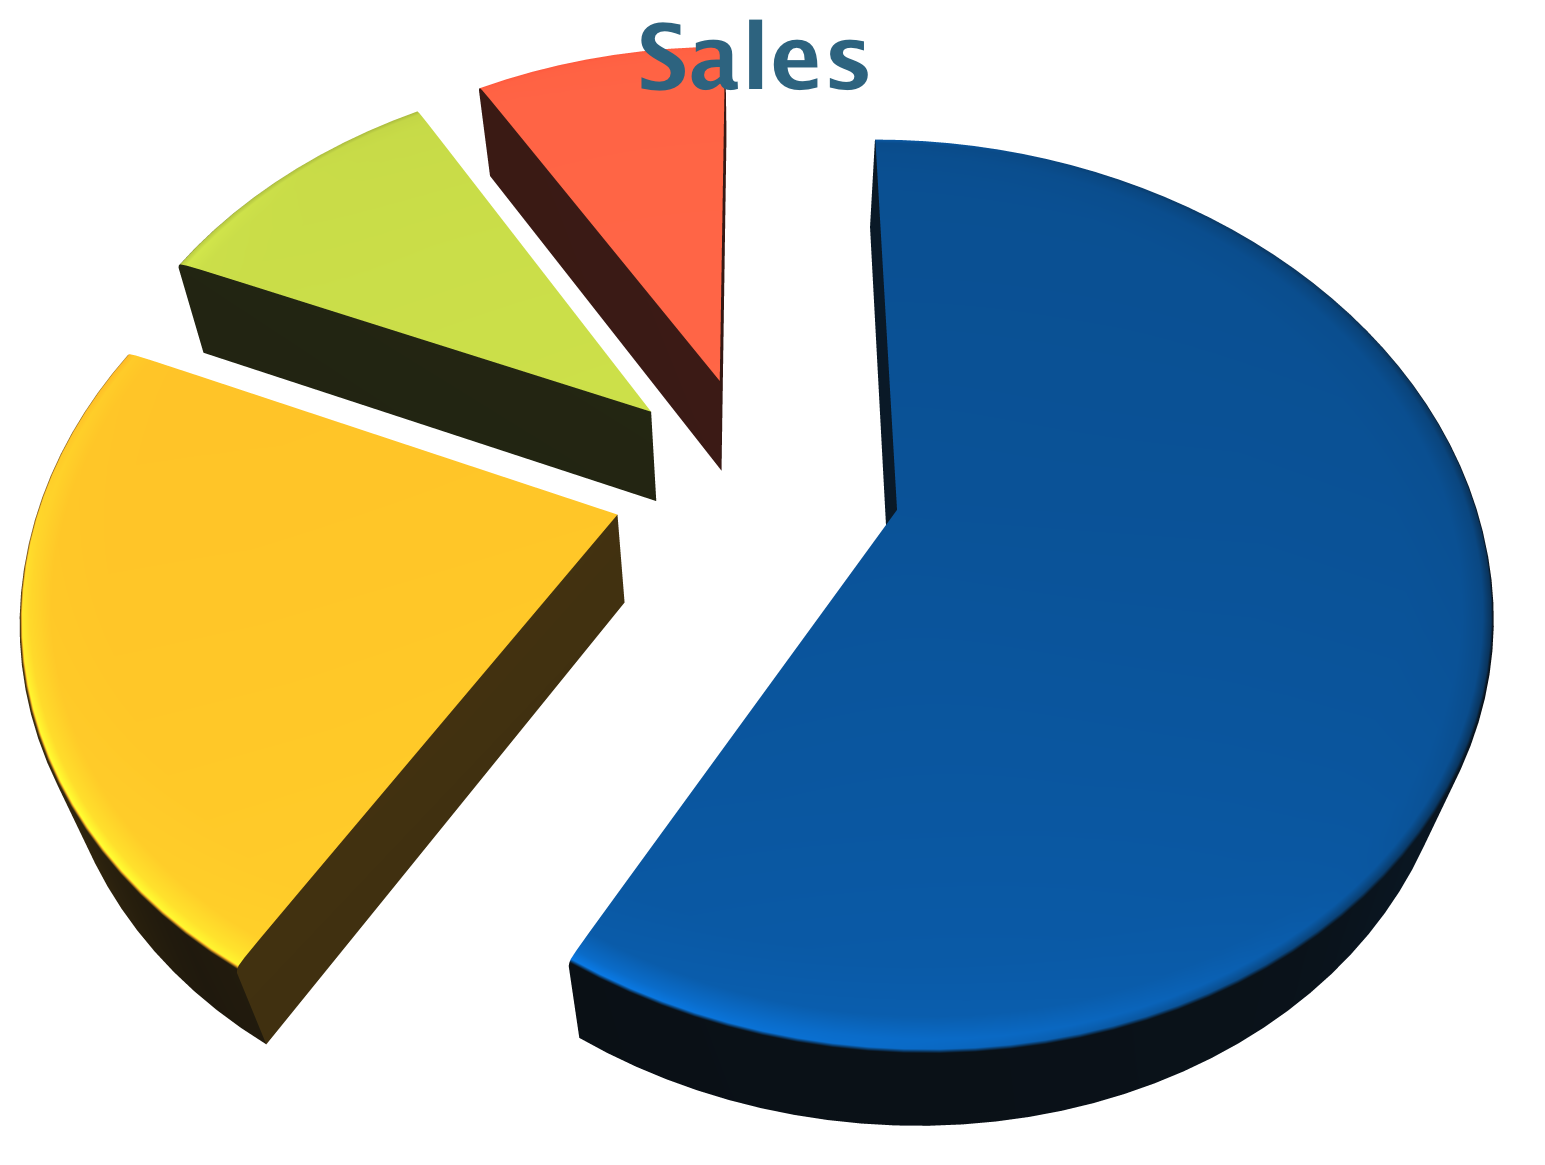
\includegraphics[width=0.4\textwidth]{chart}
\caption{\label{fig:your-figure}Caption goes here.}
\end{figure}
\end{frame}

\begin{frame}
\frametitle{Text in Two Columns}

\begin{columns}[T]

\begin{column}{0.48\textwidth}
\small
Lorem ipsum dolor sit amet, consectetur adipiscing elit. Fusce sit amet massa in dolor pellentesque tempor. Integer nunc. 
\end{column}

\begin{column}{0.48\textwidth}
\begin{itemize}
\item First bullet goes here
  \begin{itemize}
  \item Secondary bullet goes here
    \begin{itemize}
    \item Tertiary bullet goes here
    \end{itemize}
  \end{itemize}
\end{itemize}
\end{column}

\end{columns}
\end{frame}



\begin{frame}
\frametitle{Lorem Ipsum}


\includegraphics[width=.65\textwidth,height=.5\textheight]{photo}

\end{frame}


\end{document}
